The TJ-Monopix1 is one of the chips fabricated by ToweJazz with 180 CMOS imaging process. Starting from the middle of 2010 (inteso come decina) a program with the goal to find a CMOSS sensor suitable for future upgrade of experiments; a dedicated collaboration, RD53 ('Development of pixel readout integrated circuits for extreme rate and radiation'), has been estabilished in 2013 specifically for the HL-LHC Atlas and CMS detector upgrades. \\
Among the main objects of study of the collaboration there are both hybrid pixels and CMOSS MAPS: fig \ref{fig:TJ180nm} shows the intermediate steps in the MAPS research timeline.\\
Besides the Monopix series also the small electrode demonstrator TJ-Malta and mini-Malta have been produced and tested\cite{MALTA}: differently from TJ-Monopix column-drain readout, an asynchronous readout without any distribution of BCID and therefore without timestamp is used by TJ-Malta in order to reduce power consumption.

Not only TowerJazz, but also LFoundry, with the same intention, fabricated an other similar sensor with 150 CMOSS thecnology\cite{LF-Monopix}\cite{LF-TJ-Monopix}: LF-Monopix\\
The main difference between the LFoundry and TowerJazz's products, summerized in \ref{tab:LF-TJ-Monopix}, is the sensor structure rather than the read out architecture that has adopted a column drain R/O with ToT capability (LF-Monopix has 8 bits dedicated and TJ-Monopix 6 bits). Concerning the sensor, LFoundry pixels are bigger and have a large-fill factor, while TJ-Monopix has a small fill-factor electrode.\\
The performances of both the detectors have been tested before and after irradiation ($\sim 10^{10} n_{eq}/cm^{2}$) and the result is, as expected since LF-Monopix is a large fill factor electrode (capitolo \ref{chap:}), that LF-Monopix is more radiation hard than TJ-Monopix; concerning the second one the main degradation of efficiency is due to the low electic field in the pixel corner. \\
On the other side LF-Monopix1 showed a crosstalk problem principally due to the large fill-factor size ($\sim$ 55 $\%$) that influenced the pixel layout forcing the analog and digital power domain to be separate and also to be 
LF1 ha problemi di crosstalk, quindi ha bisogno di un sistema di anelli di guardia (p-stop). Ha un deep p well che è estesissimo, quindi ha anche una capacità alta. QUindi crosstalk. \\

\begin{figure}[h!]
    \centering
    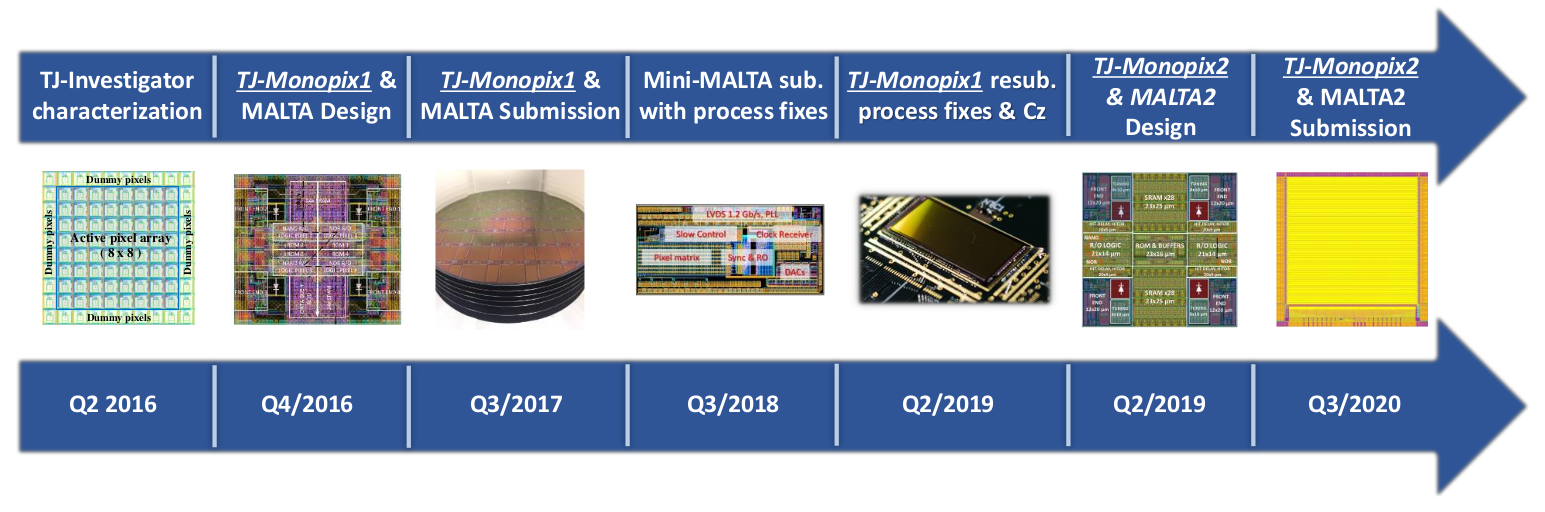
\includegraphics[width=.95\linewidth]{figures/Monopix1/TJ180nm.png}
    \caption{Timeline between the firt demonstrator TJ-investigator and TJ-Monopix2, the successor of TJ-Monopix-1.}
    \label{fig:TJ180nm}
\end{figure} 

\begin{table}
    \begin{center}
    \begin{tabular}{|c | c |c |}
    \hline
    & LF-Monopix & TJ-Monopix\\
    \hline
    \hline
    Bulk & p-type substrate & p-epi. on a low $\rho$ substrate \\
    Resistivity & $maggiore$ 2k$\Omega$cm & maggiore 1k$\Omega$cm\\
    Pixel size & 50 x 250 $\mu m^2$ & 26x40 $\mu m^2$ \\
    Depth & 100-750 $\mu$m & 25 $\mu$m \\
    Capacity & $\sim$ 400 fF & $\sim$ 3 fF\\
    Preamplifier & CSA & Voltage \\
    Threshold trimming & on pixel (4-bit DAC) & global threshold\\
    Readout mode & Fast column drain & Fast column drain\\
    Consumption & $\sim$ 300 mW/$cm^2$& $\sim$ 120 mW/$cm^2$ \\
    Threshold & 1500 $e^-$ & $\sim$ 270 $e^-$ \\
    ENC & 100 $e^-$ & $\sim$ 30 $e^-$\\
    \hline
    \end{tabular}
    \caption{Main characteristics of TJ-Monopix and LF-Monopix \cite{LF-TJ-Monopix}}
    \label{tab:LF-TJ-Monopix}
    \end{center}
 \end{table}

\section{The sensor}
    \begin{table}
        \begin{center}
        \begin{tabular}{| c |c |}
        \hline
        Parameter & Value\\
        \hline
        \hline
        Matrix size & \\
        Pixel size & 26x40 $\mu m^2$\\
        Depth & 25 $\mu$m \\
        BCID & 40 MHz \\
        ToT-bit & 6 \\
        Power consumption & $\sim$ 120 mW/$cm^2$\\
        \hline
        \end{tabular}
        \caption{}
        \label{tab:LF-TJ-Monopix}
        \end{center}
    \end{table}
    TJ-Monopix1 adopted the modification I've told about in \ref{chap:} that allows to achive a full depletion: a planar low dose n implant is build on a high resistivity ($\geq $ 1 k$\Omega$ cm), p-type epitaxial layer.\\
    The modification improves a lot the performances of the detector, especially after radiation, but  Technology Computer Aided Design (TCAD) simulations(fig.\ref{fig:Monopix1_section_scheme}) have shown that a non uniform electric field is still produced in the substrate after the modification; since the lateral component of the electric field drops at the pixel corner (this point in figure is indicated by a star) the efficiency at the side is reduced. \\
    In some cases, then, a second modification have been made to increase the lateral component of electric field: a portion of low dose implant has been removed creating a discontinuity in the pixel corner. Questo migliora le prestazioni del rivelatore, ma dall'altra parte non rende più possibile fornire tensione separatamente a deep p well e substrate, sennò si ha punchthrought.
    \begin{figure}[h!]
        \centering
        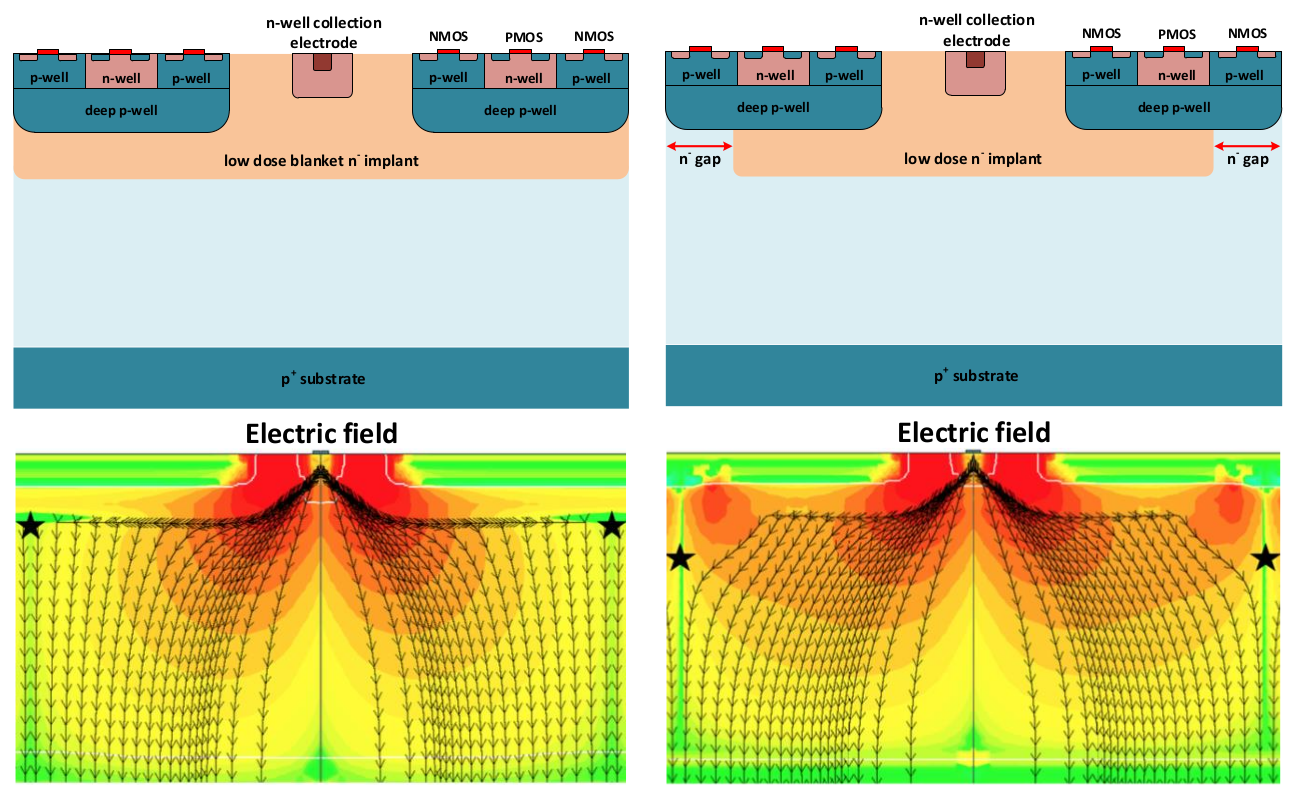
\includegraphics[width=.9\linewidth]{figures/Monopix1/Monopix1_section_scheme.png}
        \caption{(a) The cross-section of a monolithic pixel in the TJ-Monopix 180 nm with modified process; additionaly in (b) a gap in the low dose implant is created to improve the collection of charge due to a bigger lateral component of the electric field}
        \label{fig:Monopix1_section_scheme}
    \end{figure}

    Moreover, to investigate the differences in charge collection efficiency, there is a difference between pixels within the matrix: rows from 0 to 111 are fully covered by deep p-well (FDPW) under p-well near the sensor, while rows from 112 till the last 223 have a portion of deep p-well removed (RDPW). \\
    The removing enhance the the lateral electric field component then resulting in a higher efficiency, as we'll see later.\\

\section{FE flavors}
    TJ-Monopix1 has been implemented in four different flavors, each one corresponding to a different sector on the matrix (fig. \ref{fig:Monopix1_flavors}) and thus having a separate readout and data trasmission, in order to explore different variations of the FE. The four flavors mainly differ in the reset input circuit.
    \begin{figure}[h!]
        \centering
        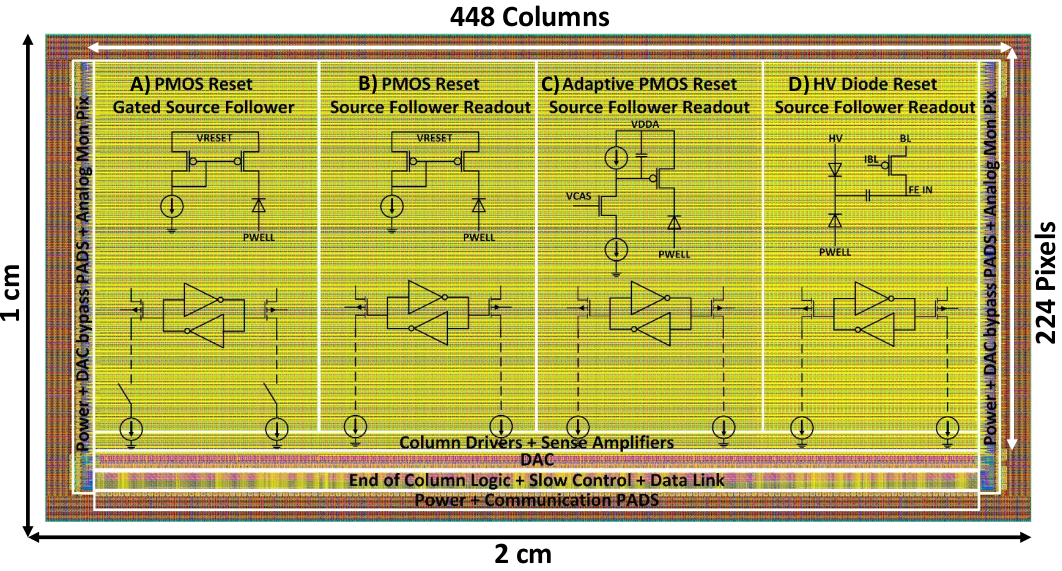
\includegraphics[width=.5\linewidth]{figures/Monopix1/Monopix1_flavors.png}
        \caption{}
        \label{fig:Monopix1_flavors}
    \end{figure}
    R resistenza di reset deve essere abbastanza grande in modo da far si che il ritorno allo zero è abbastanza lento (non devi "interferire" con la tot slope e non devi più corto del tempo del preamplificatore, sennò hai perdita di segnale).\\
    Baseline reset: all'input solitamente hai un PMOSS o un diodo;  

    The FE circuit \ref{fig:Monopix1_FE_circuit} is ALPIDE-like, so it is similar to the one described in \ref{chap:}; a quanto già detto voglio però aggiungere due parole: come viene implementato il mascheramento dei pixels e il reset.\\ 
    Prevedere un modo di mascherare gli screaming pixel, tipicamente pixels con manufacturing defects, è fondamentale per poter ridurre il rate molto alto di dati e non saturare la banda. 
    \begin{figure}[h!]
        \centering
        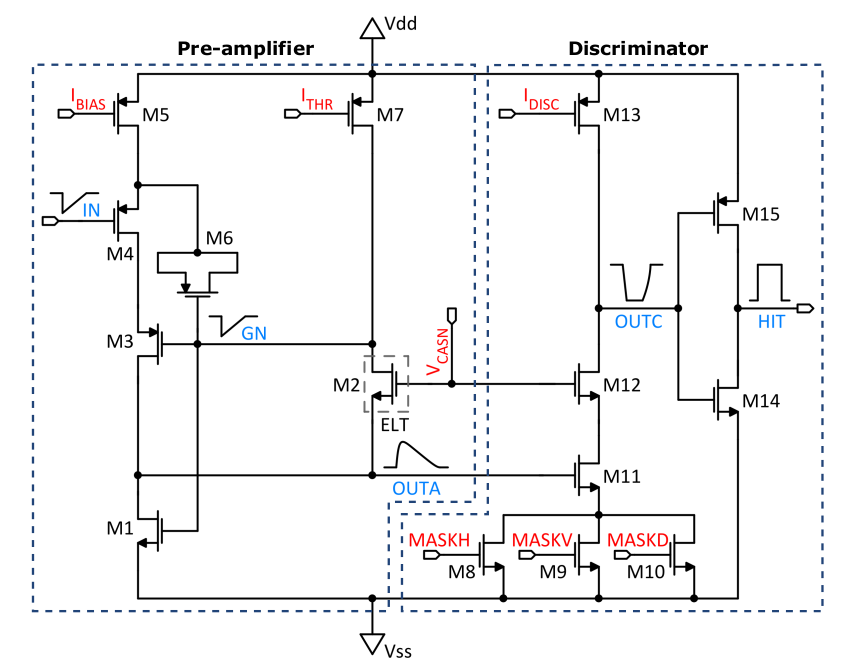
\includegraphics[width=.6\linewidth]{figures/Monopix1/Monopix1_FE_circuit.png}
        \caption{}
        \label{fig:Monopix1_FE_circuit}
    \end{figure}

    In the circuit in fig. \ref{fig:Monopix1_FE_circuit} transistors M8, M9 and M10 implement are used to disable pixels-readout, where MASKH, MASKV and MASKD represent respectivelly the vertical, orizontal and diagonal coordinates of the pixel that one want to mask. \\ 
    If all three transistors-signals are low, the discriminator is disabled and the pixel is masked. The masking is implemented in this way (with three cordinates instead of one) in order to avoid masking too many ghost pixels (fig. \ref{fig:masking_scheme}).
    \begin{figure}[h!]
        \centering
        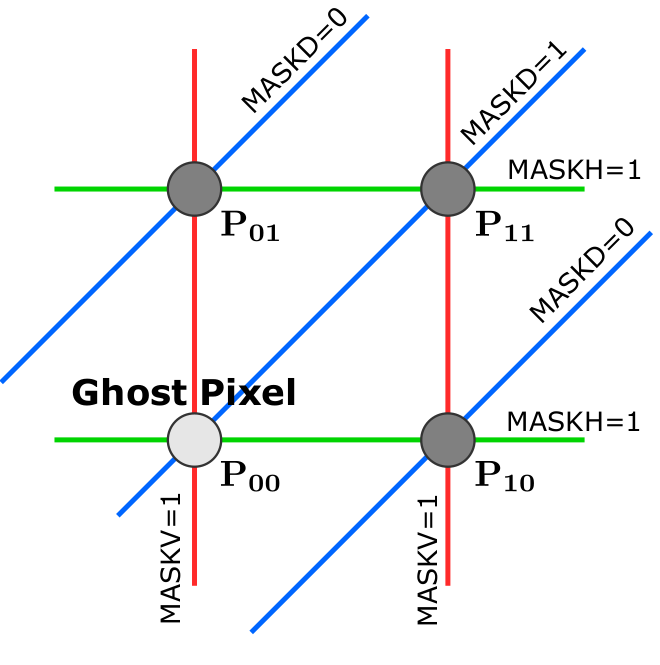
\includegraphics[width=.3\linewidth]{figures/Monopix1/masking_scheme.png}
        \caption{}
        \label{fig:masking_scheme}
    \end{figure}
    Un modo standard che si usa di solito è allocare un registro su ogni pixel periphery: il vantaggio di questo modo è che si può disabilitare ogni pixel individually. Questo metodo pur essendo più comodo richieda less amount of area ha però come drawback che il registro può essere soggetto a SEU \footnote{SEU = Single Event Upset, in sostanza è quando un bit ti cambia valore (da 0 a 1 o viceversa) perché una particella deposita carica nell'elettronica che fa da memoria (registro/RAM/...). Questo tipo di elettronica ha bisogno di un sacco di carica prima che il bit si "flippi" (cambi valore), infatti tipicamente per avere un SEU non basta una MIP che attraversa esattemente quel pezzo di chip in cui è implementata la memoria, ma un adrone che faccia interazione nucleare producendo più carica di quanto farebbe una MIP.} problema non trascurabile in acceleratori come HL-LHC adronici\\
    The implemented approch of masking in Monopix-1 funziona però solo se il numero di pixel da mascherare non è troppo alto dato che il numero di pixel unintentionally masked ("ghost pixels") increase with the number of pixels masked. \\
    Nel caso in cui solo due cordinate vengono utilizzate il numero di pixel unintentionally masked scales with $N^2$, where N is the number of the intentionally masked; if instead three coordinates are given the ghost pixels are $N^\alpha$ where $\alpha \min$2.\\

    \subsection{FE parameters}
    Descrivo un po' le misure fatte sul fe e sul significato dei vari parametri.\\
    \begin{table}
        \begin{center}
        \begin{tabular}{|c | c |}
        \hline
        Parameter & Meaning\\
        \hline
        \hline
    
        \hline
        \end{tabular}
        \caption{}
        \label{tab:FE-parameters}
        \end{center}
     \end{table}
    
\section{Readout logic and Data-packets structure}
    TJ monopix ha un colum drain readout proven by the ATLAS FEI3 front end chip (
    I. Peric et al., The FEI3 readout chip for the ATLAS pixel detector,
    Nucl. Instrum. Meth. A 565 (2006) 178, ed. by J. Grosse-Knetter, H. Krueger, and N. Wermes
    (cit. on pp. 42, 50, 60))\\

    TJ-Monopix is a triggerless. It sends data whenever it gets hits. Only thing we can do is to record timetamp of the external triggers and correlate with the hits. 
    \begin{figure}[h!]
        \centering
        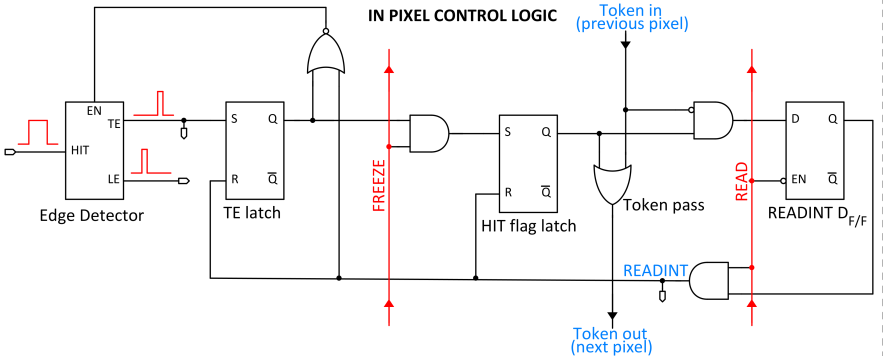
\includegraphics[width=.7\linewidth]{figures/Monopix1/Monopix1_readout_schematics.png}
        \caption{}
        \label{fig:Monopix1_readout_schematics}
    \end{figure}

    La lettura si può descrivere come una macchiana a stati in cui gli stati possibili sono READ, WAIT, DATA TRASMISSION\\

    
    \subsection{Dead time measurement}
    Descrivo come ho fatto il test. 
    Fattore limi
    \begin{figure}[h!]
            \centering
            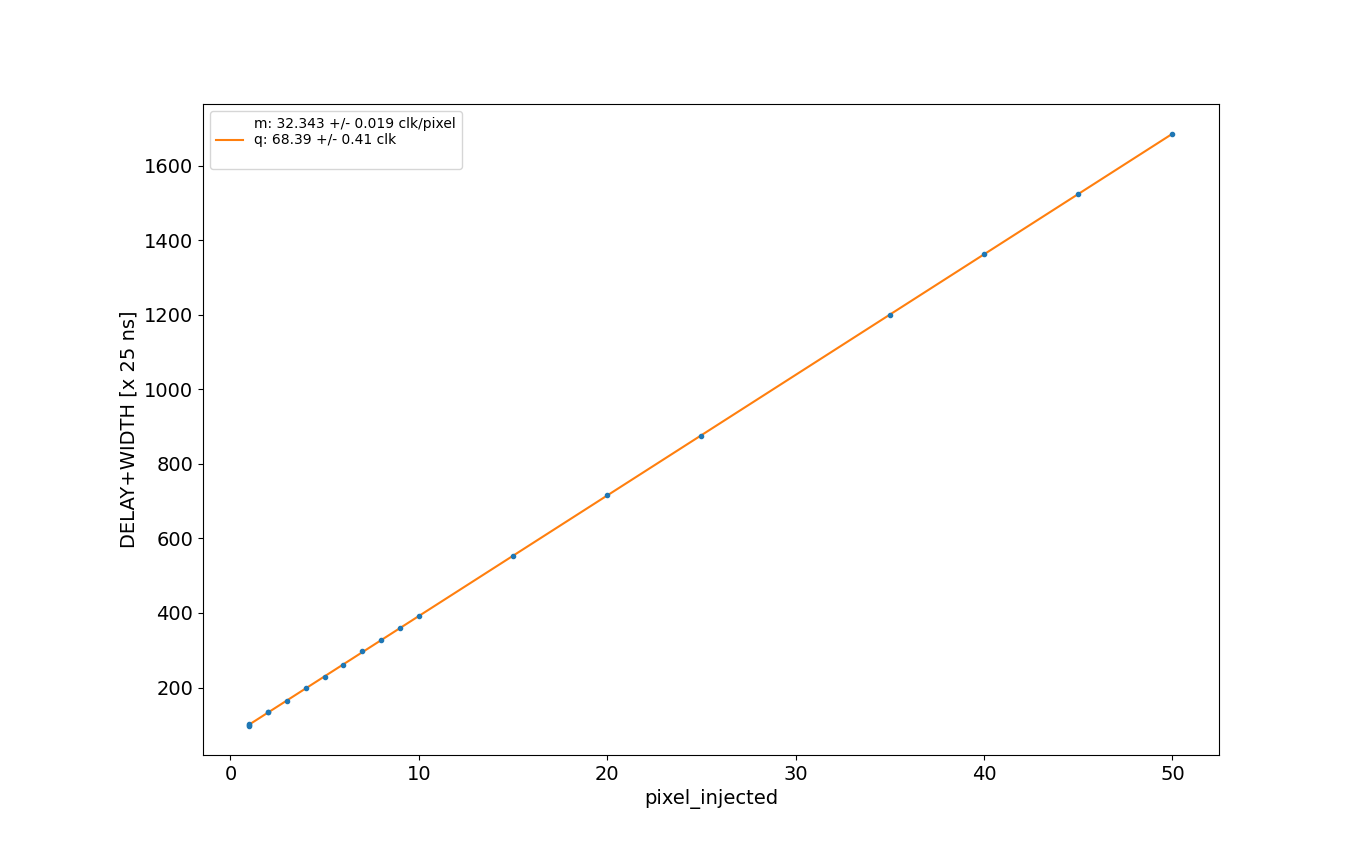
\includegraphics[width=.7\linewidth]{figures/Monopix1/dead_time.png}
            \caption{}
            \label{fig:dead_time}
        \end{figure}

    
